\chapter{Deeltjesfysica}\label{ch:b3:particle-physics}

% Provenance (not for print): second half of the "physique subatomique"
% module common to the surveyed third-year curricula: standard model
% inventory, interactions, conservation laws, detectors.

Ontdoe de materie laag voor laag van haar structuur --- moleculen, atomen,
kernen, nucleonen --- en het pellen houdt abrupt op bij een korte lijst:
zes \emph{\omterm{def:b3:particle-physics:zoo}{quarks}}, zes \emph{\omterm{def:b3:particle-physics:zoo}{leptonen}}, een handvol krachtdragers,
en één verlegen scalair die in 2012 werd gevonden. Alles wat u ooit hebt aangeraakt is
drie posten van die lijst; de rest leefde in de eerste microseconde van
het heelal en leeft weer even, overal waar
$E = mc^2$ volledig wordt betaald --- botsingen van kosmische straling en
versnellerringen. Dit hoofdstuk maakt de inventaris op: de deeltjes, de vier
wisselwerkingen die ze bewegen, de behoudswetten
(de noetherstromen van \cref{ch:b3:lagrangian-mechanics}, die nu de
subatomaire boekhouding voeren), en de detectoren die het allemaal fotograferen. Het
eindigt op uw eigen zolder, met het tellen van muonen die tien kilometer hoger zijn gemaakt.

\section{De inventaris}

\begin{definition}[Leptonen, quarks, hadronen]\label{def:b3:particle-physics:zoo}
\index{lepton}\index{quark}\index{hadron}\index{baryon}\index{meson}\index{antideeltje}
De bouwstenen van de materie zijn fermionen met spin $\tfrac12$
(\cref{ch:b3:spin-two-level}, \cref{ch:b3:identical-particles}) in
twee families van zes. \emph{Leptonen} voelen de sterke kracht niet: het
elektron, het muon en de tau (lading $-e$, elk zwaarder dan de vorige)
en hun drie neutrino's --- vrijwel massaloos, vrijwel
niet te detecteren. \emph{Quarks} komen in zes smaken --- up, down,
strange, charm, bottom, top --- met ladingen $+\tfrac23e$ (u, c,
t) en $-\tfrac13e$ (d, s, b), en zij worden nooit alleen gezien:
\emph{opsluiting} bindt ze tot \emph{hadronen} --- \emph{baryonen} van
drie quarks (proton $=$ uud, neutron $=$ udd) en
\emph{mesonen} van een quark en een antiquark (pion, kaon). Elk deeltje heeft een
\emph{antideeltje} met dezelfde massa en tegengestelde ladingen
(\cref{exo:b3:particle-physics:8}). Gewone materie gebruikt alleen de
eerste generatie --- u, d, e, $\nu_{\text{e}}$; de twee zwaardere
kopieën verschillen, voor zover iemand weet, alleen in massa. ``Wie
heeft dat besteld?'' vraagt de fysica nog steeds.
\end{definition}

\begin{omfigure}
\begin{tikzpicture}[scale=0.98,
  cell/.style={draw, minimum width=1.28cm, minimum height=1.05cm,
    font=\scriptsize, align=center, inner sep=1pt}]
  % quarks (2x3)
  \foreach \i/\n/\m in {0/u/{$+\tfrac23$}, 1/c/{$+\tfrac23$}, 2/t/{$+\tfrac23$}}
    \node[cell, fill=omDef!18] at (1.4*\i,1.1) {\textbf{\n}\\\m};
  \foreach \i/\n/\m in {0/d/{$-\tfrac13$}, 1/s/{$-\tfrac13$}, 2/b/{$-\tfrac13$}}
    \node[cell, fill=omDef!18] at (1.4*\i,0) {\textbf{\n}\\\m};
  % leptons
  \foreach \i/\n in {0/{e}, 1/{$\mu$}, 2/{$\tau$}}
    \node[cell, fill=omExo!20] at (1.4*\i,-1.35) {\textbf{\n}\\$-1$};
  \foreach \i/\n in {0/{$\nu_{\text{e}}$}, 1/{$\nu_\mu$}, 2/{$\nu_\tau$}}
    \node[cell, fill=omExo!20] at (1.4*\i,-2.45) {\textbf{\n}\\$0$};
  % bosons
  \node[cell, fill=omThm!15] at (5.0,1.1) {\textbf{g}\\sterk};
  \node[cell, fill=omThm!15] at (5.0,0) {\textbf{$\gamma$}\\EM};
  \node[cell, fill=omThm!15] at (5.0,-1.35) {\textbf{W, Z}\\zwak};
  \node[cell, fill=omThm!15] at (6.5,1.1) {\textbf{H}\\higgs};
  % generation labels
  \node[font=\scriptsize, anchor=south] at (0,1.75) {1e};
  \node[font=\scriptsize, anchor=south] at (1.4,1.75) {2e};
  \node[font=\scriptsize, anchor=south] at (2.8,1.75) {3e};
  \node[font=\scriptsize, anchor=south] at (5.75,1.75) {dragers};
  \node[font=\scriptsize, rotate=90, anchor=south] at (-1.05,0.55) {quarks};
  \node[font=\scriptsize, rotate=90, anchor=south] at (-1.05,-1.9) {leptonen};
\end{tikzpicture}

{\small De bezetting van het standaardmodel (ladingen in eenheden van $e$). Eén
kolom ervan bouwt elk atoom; de andere twee zijn dure
echo's. De zwaartekracht, bij deze massa's onmetelijk zwak, heeft geen
plaats aan tafel --- de beroemdste vacature van het model.}
\end{omfigure}

\begin{remark}[Vier wisselwerkingen]\label{rem:b3:particle-physics:forces}
\index{sterke wisselwerking}\index{zwakke wisselwerking}\index{elektrozwak}
Elk proces is een van de vier krachten aan het werk, elk gedragen door zijn
boson. De \emph{sterke} kracht (gluonen) grijpt \omterm{def:b3:particle-physics:zoo}{quarks} met een
potentiaal die met de afstand \emph{groeit} --- trek twee \omterm{def:b3:particle-physics:zoo}{quarks}
uit elkaar en het uitgerekte veld knapt tot een vers
quark-antiquarkpaar (\cref{exo:b3:particle-physics:1}): vandaar
de opsluiting, en een restant ervan lijmt kernen
(\cref{ch:b3:nuclear-physics}). Het \emph{elektromagnetisme} (het foton,
massaloos: oneindige dracht) drijft de chemie en het licht. De
\emph{zwakke} kracht (W en Z, massief met
$\approx80$--$\qty{91}{GeV}$: dracht $10^{-3}\,\unit{fm}$,
vandaar ``zwak'') is de enige die van smaak verandert --- $\beta$-verval is
een \omterm{def:b3:particle-physics:zoo}{d-quark} dat een u wordt
(\cref{prop:b3:particle-physics:conservation}) --- en de enige
kracht waarop neutrino's antwoorden. De \emph{zwaartekracht} is tussen twee protonen
$10^{36}$ keer zwakker dan het elektromagnetisme en speelt in het laboratorium
geen rol --- en toch zal zij, onafgeschermd en van lange dracht,
heel \cref{ch:b3:astrophysics} beheersen. Het elektromagnetisme en de zwakke
kracht verenigen zich bij hoge energie tot één \emph{elektrozwakke}
wisselwerking --- bij onze koude energieën uiteengedreven door de
\omterm{def:b3:phase-transitions:order}{symmetriebreking} van het higgsveld (\cref{exo:b3:particle-physics:9}).
\end{remark}

\section{De boekhouding: behoudswetten}

\begin{proposition}[Behoudswetten van deeltjesreacties]\label{prop:b3:particle-physics:conservation}
\index{baryongetal}\index{leptongetal}\index{behoudswetten!deeltjes}
Een reactie vindt alleen plaats als de boeken kloppen. Altijd
behouden: energie en impuls
(\cref{ch:b3:relativistic-dynamics}), impulsmoment en
elektrische lading --- met telkens het theorema van Noether
(\cref{thm:b3:lagrangian-mechanics:noether}) als onderbouwing.
Behouden in elke tot nu toe waargenomen reactie: het \emph{\omterm{prop:b3:particle-physics:conservation}{baryongetal}}
$B$ (\omterm{def:b3:particle-physics:zoo}{baryonen} $+1$, antibaryonen $-1$) en het \emph{\omterm{prop:b3:particle-physics:conservation}{leptongetal}}
$L$ (per familie, tot op uitstekende nauwkeurigheid). Zo heeft het proton, het
lichtste \omterm{def:b3:particle-physics:zoo}{baryon}, nergens om naartoe te vervallen --- de stabiliteit van de materie is
een boekhoudstelling --- en moet $\beta$-verval een
antineutrino meesturen:
\[
\text{n} \;\to\; \text{p} + \text{e}^- + \bar\nu_{\text{e}}
\qquad (\text{quarkniveau: } \text{d} \to \text{u} +
\text{e}^- + \bar\nu_{\text{e}}) ,
\]
wat $L$ in evenwicht brengt (en het continue energiespectrum van het elektron
verklaart, dat de fysica bijna haar geloof in energiebehoud
kostte voordat Pauli het neutrino uitvond om het te redden).
Smaken (strangeness, charm) worden door sterke en
elektromagnetische processen behouden maar \emph{door de zwakke gebroken}: vreemde
deeltjes worden overvloedig in paren geboren en sterven dan langzaam en alleen
--- de kloof van $10^{13}$ tussen sterke levensduren van $\qty{e-23}{s}$
en zwakke van $\qty{e-10}{s}$ is de vingerafdruk van de kracht die
het verval ondertekende.
\end{proposition}
\admitted

\begin{omfigure}
\begin{tikzpicture}[scale=1.0]
  % neutron -> proton beta decay quark diagram
  % three quark lines left to right
  \draw[omDef, thick] (0,2.0) -- (7.2,2.0);
  \draw[omDef, thick] (0,1.45) -- (7.2,1.45);
  \draw[omDef, thick] (0,0.9) -- (3.3,0.9);
  \draw[omThm, thick] (3.3,0.9) -- (7.2,0.9);
  \node[omDef, font=\scriptsize, anchor=east] at (-0.1,2.0) {u};
  \node[omDef, font=\scriptsize, anchor=east] at (-0.1,1.45) {d};
  \node[omDef, font=\scriptsize, anchor=east] at (-0.1,0.9) {d};
  \node[omThm, font=\scriptsize, anchor=west] at (7.3,0.9) {u};
  \node[font=\scriptsize, anchor=west] at (7.3,1.45) {d};
  \node[font=\scriptsize, anchor=west] at (7.3,2.0) {u};
  % W boson wavy-ish (zigzag)
  \draw[omExo, thick] (3.3,0.9)
    -- (3.75,0.55) -- (4.05,0.75) -- (4.35,0.35) -- (4.65,0.55)
    -- (4.95,0.15) -- (5.25,0.35) -- (5.55,-0.05);
  \node[omExo, font=\scriptsize, anchor=west] at (4.75,0.72) {W$^-$};
  % electron and antineutrino
  \draw[thick] (5.55,-0.05) -- (7.2,0.25);
  \draw[thick] (5.55,-0.05) -- (7.2,-0.55);
  \node[font=\scriptsize, anchor=west] at (7.3,0.25) {e$^-$};
  \node[font=\scriptsize, anchor=west] at (7.3,-0.55) {$\bar\nu_{\text{e}}$};
  % braces labels
  \node[font=\scriptsize, anchor=east] at (-0.75,1.45) {neutron};
  \node[font=\scriptsize, anchor=west] at (8.35,1.45) {proton};
\end{tikzpicture}

{\small $\beta$-verval, ingezoomd tot op het quarkniveau: één \omterm{def:b3:particle-physics:zoo}{d-quark}
wordt een u door een virtuele W$^-$ uit te zenden, die zich als
elektron plus antineutrino materialiseert. Alle boeken kloppen: lading
$-\tfrac13 = +\tfrac23 - 1 + 0$, \omterm{prop:b3:particle-physics:conservation}{baryongetal}, \omterm{prop:b3:particle-physics:conservation}{leptongetal}.}
\end{omfigure}

\section{Deeltjes maken en zien}

\begin{remark}[Versnellers en detectoren]\label{rem:b3:particle-physics:machines}
\index{botser}\index{deeltjesdetector}
Twee redenen om te versnellen: \emph{oplossend vermogen} --- een sonde ziet geen
detail fijner dan haar golflengte $\lambda = h/p$
(\cref{ch:b3:crystalline-solids} gebruikte ångströms; femtometers
kosten \unit{GeV}'s) --- en \emph{schepping}: botsingsenergie
wordt nieuwe massa, en twee bundels frontaal laten botsen besteedt haar helemaal
(een vast trefplaatje verspilt het meeste ervan aan het meevoeren van het puin:
\cref{exo:b3:particle-physics:4}). Ringvormige botsers laten dezelfde
deeltjes telkens opnieuw door dezelfde versnelspleet gaan terwijl
magneten ze sturen --- ten koste van synchrotronstraling
$\propto\gamma^4$, en daarom laat de ring die de higgs vond
zware protonen botsen en geen vederlichte elektronen. Rond het
kruispunt liggen uienlagen, die elk één vraag stellen: een
\emph{spoorzoeker} buigt geladen banen in een magneet (impuls); een
elektromagnetische \emph{calorimeter} slikt elektronen en
fotonen (energie); een hadronische slikt pionen en protonen;
en alleen muonen slaan door tot de buitenste kamers ---
identiteit naar begraafdiepte. Neutrino's vertrekken als ontbrekende
impuls: de boekhouding detecteert wat niets kan tegenhouden.
\end{remark}

\begin{omfigure}
\begin{tikzpicture}[scale=1.0]
  % quadrant onion detector
  \fill[omDef!10] (0,0) -- (4.7,0) arc (0:80:4.7) -- cycle;
  \fill[omExo!18] (0,0) -- (3.5,0) arc (0:80:3.5) -- cycle;
  \fill[omThm!12] (0,0) -- (2.3,0) arc (0:80:2.3) -- cycle;
  \fill[white] (0,0) -- (1.2,0) arc (0:80:1.2) -- cycle;
  \foreach \r in {1.2,2.3,3.5,4.7} \draw[gray] (\r,0) arc (0:80:\r);
  \draw[gray] (0,0) -- (4.7,0);
  \draw[gray] (0,0) -- (80:4.7);
  % labels of layers, along the free bottom edge
  \node[font=\tiny, anchor=north] at (1.75,-0.12) {spoorzoeker};
  \node[font=\tiny, anchor=north] at (2.9,-0.12) {em.\ cal.};
  \node[font=\tiny, anchor=north] at (4.1,-0.12) {hadr.\ cal.};
  \node[font=\tiny, anchor=west] at (12:4.85) {muonkamers};
  % particle tracks from origin
  % electron: curved, stops in ecal
  \draw[omDef, thick] (0,0) .. controls (1.1,0.62) .. (2.05,1.55);
  \fill[omDef] (2.6,1.9) circle (2pt);
  \node[omDef, font=\tiny, anchor=south west] at (2.5,1.98) {e$^-$};
  % photon: straight dashed (neutral), stops in ecal
  \draw[omDef, dashed] (0,0) -- (55:2.75);
  \fill[omDef] (55:2.95) circle (2pt);
  \node[omDef, font=\tiny, anchor=south] at (55:3.2) {$\gamma$};
  % pion: curved into hadronic
  \draw[omThm, thick] (0,0) .. controls (0.75:2.0) and (5:2.6) .. (12:3.9);
  \fill[omThm] (14:4.1) circle (2pt);
  \node[omThm, font=\tiny, anchor=north] at (10:4.28) {$\pi$};
  % muon: nearly straight, exits
  \draw[omExo, very thick] (0,0) .. controls (70:2.4) .. (73:5.2);
  \node[omExo, font=\tiny, anchor=south] at (73:5.35) {$\mu$};
\end{tikzpicture}

{\small Een botsingsdetector in doorsnede. Elke soort
schrijft haar handtekening: geladen sporen krommen in het veld van de
spoorzoeker; elektronen en fotonen sterven in de binnenste calorimeter,
\omterm{def:b3:particle-physics:zoo}{hadronen} in de buitenste; alleen muonen bereiken de verste kamers; en
wat ongezien ontsnapt --- het neutrino --- wordt van de ontbrekende
impuls afgelezen.}
\end{omfigure}

\begin{remark}[De higgs, en het open grootboek]\label{rem:b3:particle-physics:higgs}
\index{higgsdeeltje}\index{donkere materie}
De symmetrie van het standaardmodel verbiedt kale massa's voor zijn
deeltjes; het \emph{higgsveld}, dat de hele ruimte vult met een
condensaat dat van nul verschilt --- de keuze uit de dubbele put van
\cref{ch:b3:phase-transitions}, verheven tot het vacuüm zelf
--- breekt de symmetrie en verleent massa's via zijn koppelingen:
hoe zwaarder het deeltje, hoe steviger de greep. Zijn eigen kwantum, het \omterm{rem:b3:particle-physics:higgs}{higgsdeeltje}
(\qty{125}{GeV}, gevonden in 2012), maakte de tabel af. Het
open grootboek is langer: neutrino's oscilleren tussen smaken en
moeten dus massa hebben die het model nooit heeft opgeschreven
(\cref{exo:b3:particle-physics:10}); sterrenstelsels draaien alsof ze worden vastgehouden
door vijf keer meer materie dan er straalt
(\cref{ch:b3:astrophysics}); en het heelal bevat materie
maar vrijwel geen antimaterie, een asymmetrie waarvoor de piepkleine
CP-schending van het model nog niet kan betalen. De lijst is het lesprogramma van
wat er ook volgt.
\end{remark}

\begin{omfigure}
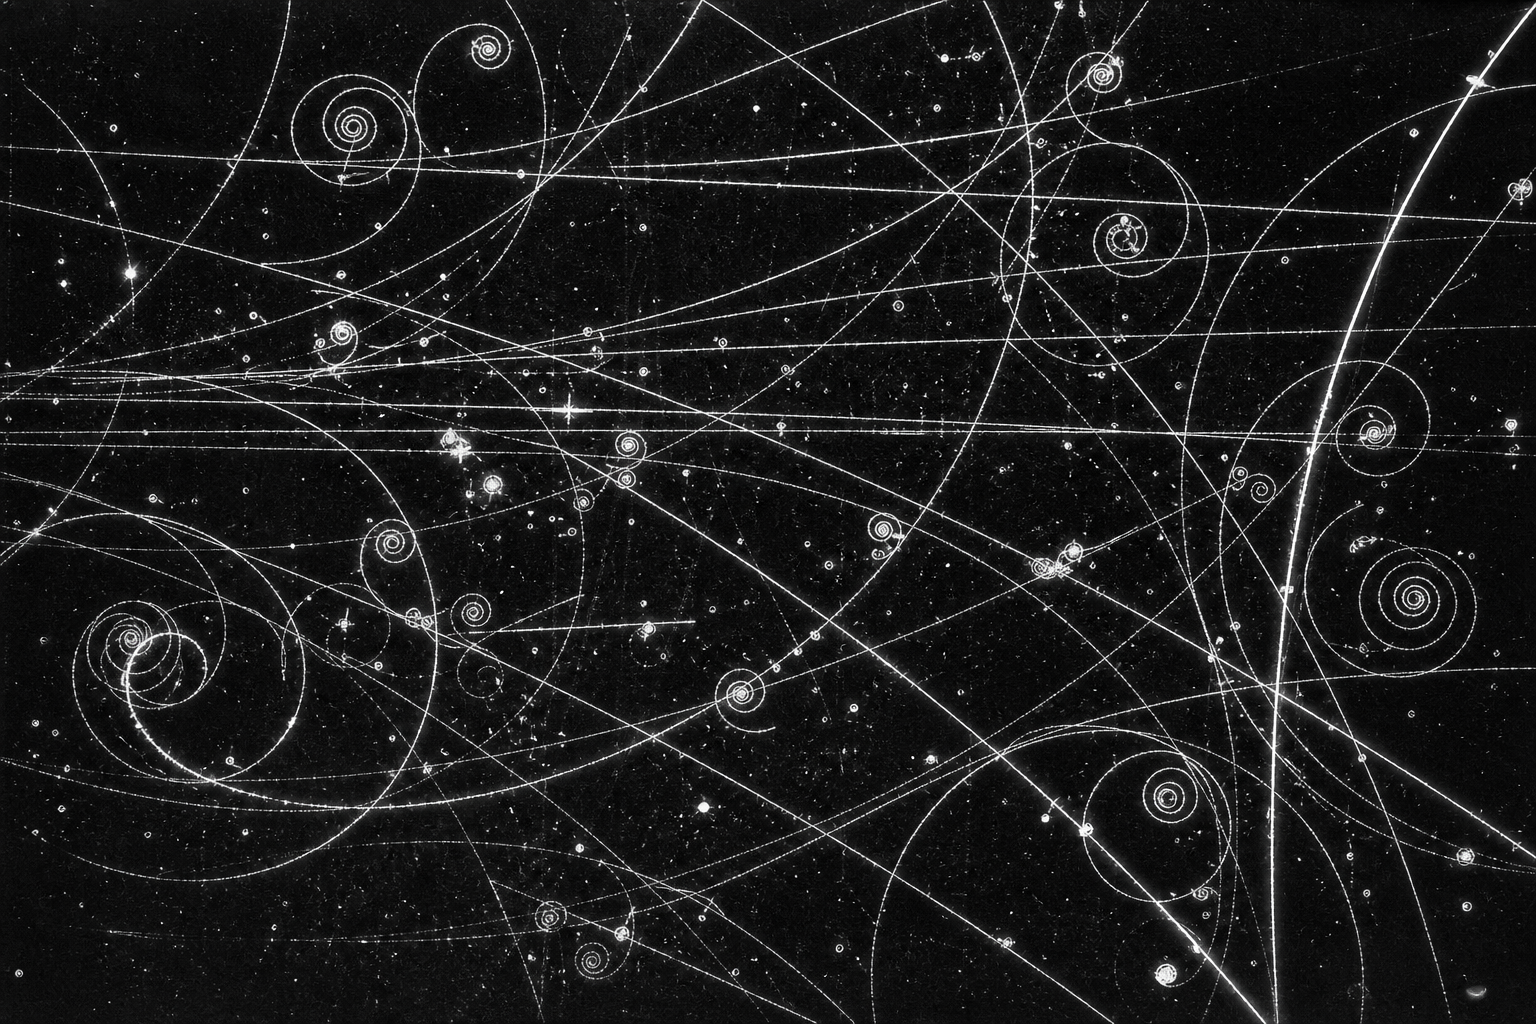
\includegraphics[width=0.58\linewidth]{images/book5/ai/b5-22-bubble-chamber-spirals.png}

{\small Een beeld uit een bellenvat: geladen sporen die in een magneetveld krullen, met elektronen en positronen die tegengesteld spiraliseren terwijl ze energie verliezen. Decennialang werd de deeltjesfysica beeldje voor beeldje van zulke film afgelezen.}
\end{omfigure}

\section{Opgaven}

\begin{exercise}[$\star$]\label{exo:b3:particle-physics:1}
Quarkrekenwerk. (a) Controleer de ladingen van p $=$ uud en
n $=$ udd. (b) Het pion $\pi^+$ is $\text{u}\bar{\text{d}}$:
controleer zijn lading. (c) Stel quarkinhouden voor voor $\pi^-$ en voor
de $\Delta^{++}$ (lading $+2e$). (d) Waarom levert een \omterm{def:b3:particle-physics:zoo}{quark} uit een proton
trekken een regen van \omterm{def:b3:particle-physics:zoo}{mesonen} op in plaats van een vrij \omterm{def:b3:particle-physics:zoo}{quark}?
\end{exercise}

\begin{exercise}[$\star$]\label{exo:b3:particle-physics:2}
Sorteren. Geef voor elk van e$^-$, $\nu_\mu$, $\pi^+$, p, n,
$\mu^-$ aan: (a) \omterm{def:b3:particle-physics:zoo}{lepton}, \omterm{def:b3:particle-physics:zoo}{baryon} of \omterm{def:b3:particle-physics:zoo}{meson}? (b) welke voelen de sterke
kracht? (c) welke zijn in isolatie stabiel? (d) welke kan een
magneetveld niet afbuigen?
\end{exercise}

\begin{exercise}[$\star$]\label{exo:b3:particle-physics:3}
Toegestaan of verboden? Beoordeel en noem de geschonden wet indien van toepassing:
(a) $\text{n} \to \text{p} + \text{e}^- + \bar\nu_{\text{e}}$;
(b) $\text{p} \to \text{n} + \text{e}^+ + \nu_{\text{e}}$ (voor
een \emph{vrij} proton);
(c) $\text{p} \to \text{e}^+ + \gamma$;
(d) $\mu^- \to \text{e}^- + \gamma$.
\end{exercise}

\begin{exercise}[$\star$]\label{exo:b3:particle-physics:4}
De prijs van de schepping. Een paar proton-antiproton maken vanuit
een protonbundel op een waterstoftrefplaatje vergt (volgens het argument met
\omterm{def:b3:relativistic-dynamics:four-momentum}{invariante massa} uit \cref{ch:b3:relativistic-dynamics}) een
kinetische bundelenergie van $6m_{\text{p}}c^2$. (a) Evalueer die in GeV.
(b) Welke kinetische energie van twee bundels volstaat in een botser voor
hetzelfde paar? (c) Bereken de verhouding van de ``verspilling'' en leg uit waar
de energie bij een vast trefplaatje heen gaat. (d) Waarom had de machine die in 1955
het antiproton ontdekte $\sim\qty{6}{GeV}$ nodig?
\end{exercise}

\begin{exercise}[$\star\star$]\label{exo:b3:particle-physics:5}
Het muon, twee keer. Het muon ($m = \qty{106}{MeV}$,
$\tau = \qty{2.2}{\micro s}$) is de zware tweeling van het elektron. (a)
Welke afstand is $c\tau$? (b) Kosmische muonen die op
\qty{15}{km} worden geboren bereiken de grond: welke $\gamma$ eist
dat overleven, en welke energie is dat? (c) Beschrijf hetzelfde overleven
vanuit het eigen stelsel van het muon. (d) Waarom vervalt het muon tot een
elektron maar nooit tot een proton, en waarom is zijn verval naar
deeltjesmaatstaven \emph{traag}?
\end{exercise}

\begin{exercise}[$\star\star$]\label{exo:b3:particle-physics:6}
Binnen in het $\beta$-verval. (a) Schrijf het neutronverval op quarkniveau
op en controleer alle behouden grootheden. (b) Het energiespectrum van het
uitgezonden elektron is continu tot een eindpunt:
leg uit hoe dit ooit het energiebehoud bedreigde en hoe
Pauli's neutrino het redde. (c) Het W-boson weegt
\qty{80.4}{GeV}: schat de dracht van de zwakke kracht
$\hbar/m_{\text{W}}c$ ($\hbar c = \qty{197}{MeV.fm}$). (d) Gebruik
die dracht om in één zin uit te leggen waarom de ``zwakke'' kracht bij lage
energie zwak is en toch elektrozwak-sterk bij hoge.
\end{exercise}

\begin{exercise}[$\star\star$]\label{exo:b3:particle-physics:7}
Vreemde boekhouding. Kaonen en $\Lambda$-hyperonen dragen een
smaak, \emph{strangeness}, die door de sterke kracht wordt behouden maar
niet door de zwakke. (a) Leg uit waarom botsingen van kosmische straling
vreemde deeltjes alleen in paren voortbrengen. (b) De $\Lambda$ leeft
$\qty{2.6e-10}{s}$ --- vergelijk met de $\qty{e-23}{s}$ van
sterke vervallen en concludeer welke kracht hem doodt. (c) Welke verhouding
van tijdschalen scheidt de twee, en met welke alledaagse verhouding is
die vergelijkbaar (één seconde tegenover wat)? (d) Hoe dwong dit
``vreemde'' gedrag --- overvloedige geboorte, aarzelende dood ---
de uitvinding van een nieuw kwantumgetal af?
\end{exercise}

\begin{exercise}[$\star\star$]\label{exo:b3:particle-physics:8}
Antimaterie, verzilverd. (a) Waarom moet
$\text{e}^+ + \text{e}^- \to \gamma$ (één foton) verboden zijn,
terwijl twee fotonen prima kunnen? (b) Bereken de energie die vrijkomt bij het
annihileren van één gram antimaterie met één gram materie, en
vergelijk die met de kilogram gespleten uranium van
\cref{exo:b3:nuclear-physics:9}. (c) PET-scanners
(\cref{exo:b3:nuclear-physics:12}) draaien op positronen: waar komen
de positronen van de geneeskunde vandaan? (d) Antiprotonen maken kost
$\sim10^{6}$ keer hun \omterm{def:b3:relativistic-dynamics:momentum-energy}{rustenergie} aan stopcontactvermogen: becommentarieer
antimaterie als brandstof.
\end{exercise}

\begin{exercise}[$\star\star\star$]\label{exo:b3:particle-physics:9}
De higgs als \omterm{def:b3:phase-transitions:order}{faseovergang}. (a) Herformuleer in de taal van
\cref{exo:b3:phase-transitions:12} wat het betekent dat het
vacuüm in een symmetriebrekende put zit. (b) Waarom krijgen de W en de Z
massa terwijl het foton massaloos blijft (welk deel van de
symmetrie overleeft)? (c) Het \omterm{rem:b3:particle-physics:higgs}{higgsdeeltje} is de radiale trilling van het
veld: wat speelt die rol in de magneet van
\cref{thm:b3:phase-transitions:meanfield}? (d) Boven
$\sim10^{15}\,\unit{K}$ wordt de symmetrie hersteld: waar en wanneer
was het heelal voor het laatst zo heet (\cref{ch:b3:astrophysics})?
\end{exercise}

\begin{exercise}[$\star\star\star$]\label{exo:b3:particle-physics:10}
Neutrino's bij de miljard. (a) De Zon maakt twee neutrino's per
cyclus $4\text{p} \to {}^4\text{He}$ (\qty{26.7}{MeV}): bereken uit de
zonneconstante \qty{1360}{W/m^2} de neutrinoflux bij de
aarde. (b) Hoeveel steken er uw duimnagel
(\qty{1}{cm^2}) per seconde over, en hoeveel zullen er ruwweg in een mensenleven
met uw lichaam wisselwerken (neem een
wisselwerkingskans van de orde $10^{-22}$ per meter vlees per neutrino als
gegeven)? (c) Vroege
detectoren vingen maar een derde van de voorspelde
$\nu_{\text{e}}$: geef de oplossing (oscillaties) en haar
structurele gevolg voor het standaardmodel. (d) Waarom woont een
neutrinodetector onder een berg?
\end{exercise}

\begin{exercise}[$\star\star\star$]\label{exo:b3:particle-physics:11}
Machinegetallen. LHC-protonen: elk $E = \qty{6.8}{TeV}$. (a)
Bereken $\gamma$ en $1 - v/c \approx 1/2\gamma^2$. (b) Welke
golflengte $\lambda \approx hc/E$ tast structuur af, en vergelijk die
met de straal van \qty{0.8}{fm} van het proton. (c) Frontale botsingsenergie:
\qty{13.6}{TeV} --- hoeveel protonrustmassa's zou die
kunnen scheppen? (d) Het synchrotronverlies schaalt als $\gamma^4$:
bereken de verhouding van $\gamma$ voor elektron en proton bij vaste energie
en onderbouw protonen voor de ring en elektronen voor precisiemachines.
\end{exercise}

\begin{exercise}[$\star\star\star$]\label{exo:b3:particle-physics:12}
Boodschappers van de rand. De kosmische straling met de hoogste energie ooit
geregistreerd droeg $\sim\qty{3e20}{eV}$ --- één enkel proton. (a)
Reken om naar joule en noem een macroscopisch voorwerp met die
kinetische energie. (b) Bereken zijn $\gamma$, en de breedte van
het Melkwegstelsel ($\sim10^{5}$ lichtjaar) in zijn eigen stelsel. (c) Boven
$\sim\qty{5e19}{eV}$ verstrooien protonen aan de kosmische achtergrondstraling
(\cref{ch:b3:photons-phonons}) --- leg
kwalitatief uit waarom het heelal ondoorzichtig voor ze is. (d) Waarom leren
zulke energieën, ver voorbij elke versneller, ons toch minder
dan de LHC doet? (Denk aan flux en beheersing.)
\end{exercise}

\begin{omfigure}
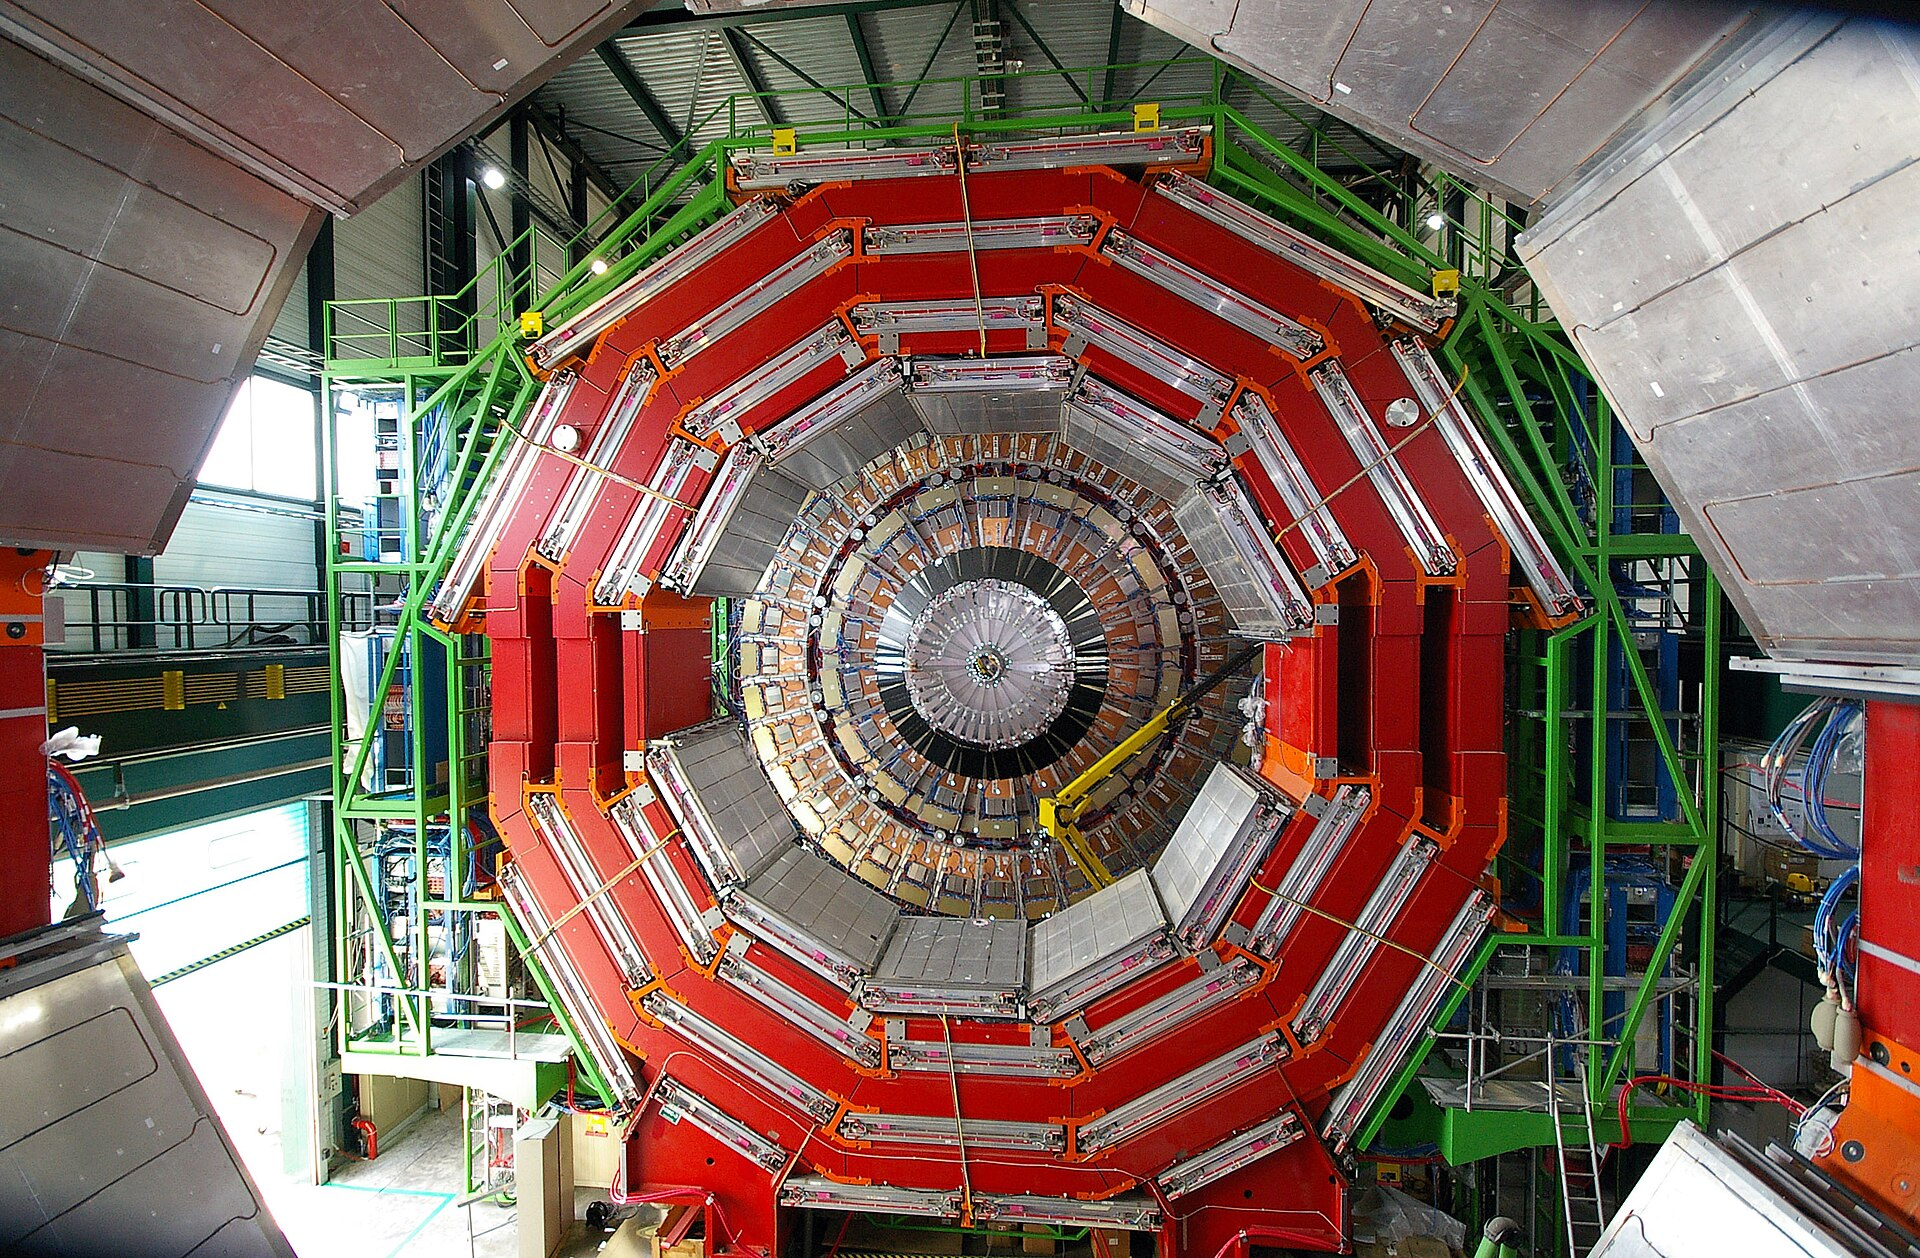
\includegraphics[width=0.62\linewidth]{images/book5/photo-cms-construction.jpg}

{\small De CMS-detector in aanbouw (foto: Julian Williams, vrij gebruik): de uienlagen van de cilinder, van voren, vóór het sluiten --- een uitvoering van vijftienduizend ton van de laatste figuur van dit hoofdstuk.}
\end{omfigure}

\section{Vraagstuk: De muontelescoop op zolder}

\begin{problem}\label{pb:b3:particle-physics:1}
\emph{De muontelescoop op zolder.} Voor de wetenschapsbeurs bouwt u een
telescoop voor kosmische straling: twee scintillatorplaten van $20\times20$\,\unit{cm},
de ene \qty{30}{cm} boven de andere, elk uitgelezen door een fotomultiplicator,
in coïncidentie geschakeld --- alleen een telling als \emph{beide}
binnen \qty{100}{ns} afgaan. Muonflux op zeeniveau door een horizontaal
oppervlak: ongeveer 1 per \unit{cm^2} per minuut.

\medskip\noindent\textbf{Deel I --- De hemel tellen.}

\begin{enumerate}
  \item Waar beginnen uw muonen? Volg de keten: primair
        proton, hogere atmosfeer, pionen, muonen --- en noem welke
        kracht elke stap beheerst.
  \item Waarom bereiken de pionen zelf vrijwel nooit de
        grond ($\tau_\pi = \qty{26}{ns}$), terwijl hun dochtermuonen
        dat wel doen?
  \item Voorspel het tempo van één plaat uit de gegeven flux.
  \item De plaat alleen klikt in werkelijkheid veel vaker ---
        elektronische ruis en omgevingsradioactiviteit
        (\cref{ch:b3:nuclear-physics}). Leg uit hoe de
        coïncidentie van twee platen daar bijna alles van doodt.
  \item Welk tempo aan toevallige coïncidenties leveren twee onafhankelijke
        ruisbronnen van \qty{100}{Hz} in een venster van \qty{100}{ns}
        op ($R_{\text{acc}} = R_1R_2\Delta t$)? Vergelijk met
        het echte muontempo.
  \item Je coïncidentietempo bezinkt rond 100 per minuut ---
        ruim onder de 400 van één plaat. Verklaar: welke muonen
        laat de meetkunde van twee platen toe?
  \item Kantel de telescoop: het tempo daalt ruwweg als
        $\cos^2\theta$ van de zenithoek. Geef de fysische
        reden (wat groeit er met $\theta$?).
\end{enumerate}

\medskip\noindent\textbf{Deel II --- Relativiteit, op zolder geverifieerd.}

\begin{enumerate}[resume]
  \item Muonen: $\tau = \qty{2.2}{\micro s}$. Bereken $c\tau$ en
        concludeer wat een \emph{klassiek} muon dat op
        \qty{15}{km} wordt geboren zou kunnen.
  \item Jouw muonen hebben gemiddeld $E \approx \qty{4}{GeV}$
        ($m_\mu c^2 = \qty{106}{MeV}$): bereken $\gamma$.
  \item De opgerekte levensduur, en het bijbehorende bereik: klopt het
        zoldertempo nu?
  \item Vertel het overleven opnieuw vanuit het stelsel van het muon
        (\cref{ch:b3:relativistic-kinematics}).
  \item Bereken voor $\gamma = 38$ de overlevende fractie vanaf
        \qty{15}{km} ($t_{\text{eigen}} = L/\gamma v$, overleving
        $\eu^{-t/\tau}$).
  \item Jouw telescoop is dus \emph{welk} klassiek
        experiment, met schoolonderdelen nagebouwd? Zeg wat een nul\-resultaat
        (klassiek verval) voor uw teller zou hebben voorspeld.
\end{enumerate}

\medskip\noindent\textbf{Deel III --- Wat een muon is.}

\begin{enumerate}[resume]
  \item Plaats het muon in de tabel van het standaardmodel: familie,
        generatie, lading, spin.
  \item Het vervalt: $\mu^- \to \text{e}^- + \bar\nu_{\text{e}} +
        \nu_\mu$. Controleer de lading en beide leptonfamiliegetallen.
  \item Waarom is het energiespectrum van het vervalelektron continu,
        en wat is zijn eindpunt ($\approx m_\mu c^2/2$)?
  \item Waarom is $\mu^- \to \text{e}^- + \gamma$ --- nooit
        waargenomen --- zo interessant voor de experimenten van vandaag?
        (Wat zou de ontdekking ervan breken?)
  \item Een muon dat in uw plaat tot stilstand komt vervalt in rust: beschrijf
        de vertraagde tweede flits en hoe die u $\tau$
        rechtstreeks aanreikt.
  \item Muonen zijn ``zware elektronen'': geef één gevolg voor
        atomen --- wat gebeurt er met de \omterm{thm:b3:hydrogen-atom:levels}{bohrstraal} van muonische
        waterstof (\cref{ch:b3:hydrogen-atom}), geschaald met
        $m_\mu/m_{\text{e}} \approx 207$?
\end{enumerate}

\medskip\noindent\textbf{Deel IV --- De keten op.}

\begin{enumerate}[resume]
  \item Een primair proton van $\qty{e15}{eV}$ brengt een lawine van
        miljoenen voort. Schat de gemiddelde energie per lawinedeeltje
        als $10^{6}$ deeltjes haar delen.
  \item Grote observatoria vervangen uw platen door honderden
        watertanks die kilometers uit elkaar staan en op
        \emph{cherenkovlicht} letten (\cref{pb:b3:nuclear-physics:1}):
        wat doen muonen in het water, en waarom staan de tanks \emph{ver
        uit elkaar}?
  \item Jouw scintillator met fotomultiplicator werkt op hetzelfde
        principe als de calorimeters bij de grote botsers:
        verwoord dat gedeelde principe in één zin
        (deeltje $\to$ licht $\to$ elektronen $\to$ tellen).
  \item Ooit deden foto's van bellenvaten het zien: geladen
        sporen die in een magneetveld krullen. Welke twee grootheden
        geeft de krul u, en welk deeltje laat helemaal geen spoor na?
  \item De recordkosmische straling van
        \cref{exo:b3:particle-physics:12} sloeg in met de energie van
        een geserveerde tennisbal in één proton. Wat zegt haar
        bestaan over de versnellers van de natuur tegenover de onze?
  \item Vat de posterpresentatie in vier regels samen: geboren uit een
        proton tien kilometer hoog, bezorgd door tijddilatatie,
        herkend aan twee gelijktijdige flitsen, en verklaard door een
        tabel met twaalf plaatsen.
\end{enumerate}
\end{problem}
